\documentclass[../../main.tex]{subfiles}

\graphicspath{{../../image/}{../../figure/}}

\begin{document}

\section{概率密度}\label{section:ch02-概率密度}

我们除了关注在离散数值集合上定义概率，还关注连续变量的概率。例如，我们可能想预测给病人服用药物的剂量。由于在预测中会有不确定性，而我们想要量化这种不确定性，因此就需要再次利用概率。然而，在无限精度下，观测到连续变量为某个特定值的概率几乎为零。为此，需要引入概率密度（probability density）的概念。这里我们只做相对非正式的讨论。

定义连续变量 $x$ 上的概率密度 $p(x)$，如\cref{figure:ch02-密度与累积分布}所示，当 $\delta x\to0$ 时，$x$ 落在区间 $(x,x+\delta x)$ 的概率由 $p(x)\delta x$ 给出。$x$ 落在区间 $(a,b)$ 的概率为

\begin{align}
  p\big(x\in(a,b)\big) = \int_{a}^{b} p(x)\,\mathrm{d}x
  \label{align:ch02-区间概率}
\end{align}

\begin{definition}[概率密度]\label{definition:ch02-概率密度}
设 $x$ 为实值连续随机变量。若存在非负函数 $p(x)$，使得当 $\delta x\to0$ 时 $x$ 落在区间 $(x,x+\delta x)$ 内的概率为 $p(x)\delta x$，则称 $p(x)$ 为 $x$ 的\textbf{概率密度}（probability density）。此时 $x$ 落在区间 $(a,b)$ 内的概率由\eqref{align:ch02-区间概率}给出。
\end{definition}

% SUPPLEMENT: parent=definition:ch02-概率密度; kind=motivation; location=紧随其后的 remark（重构新增）
\begin{remark}（重构新增）
引入密度的动机是：连续变量取任一确定值的概率为零，因此不能像离散情形那样用 $p(X=x_i)$ 来描述分布，只能用“落在一个小区间里的概率与区间长度之比”来描述。\cref{definition:ch02-概率密度}正是把这个比值固定在 $x$ 处的极限值上，于是 $p(x)$ 本身不是概率，$p(x)\delta x$ 才是概率。

条件“$\delta x\to0$”不可省：若只对某个固定的 $\delta x$ 定义，则得到的依赖于区间划分，不构成 $x$ 的函数。也正因为 $p(x)$ 是密度而非概率，它可以大于 $1$（例如 $\mathcal{N}(0,0.01)$ 在 $x=0$ 处约为 $3.99$），只有\eqref{align:ch02-区间概率}的积分才是概率。
\end{remark}

\begin{figure}[htbp]
  \centering
  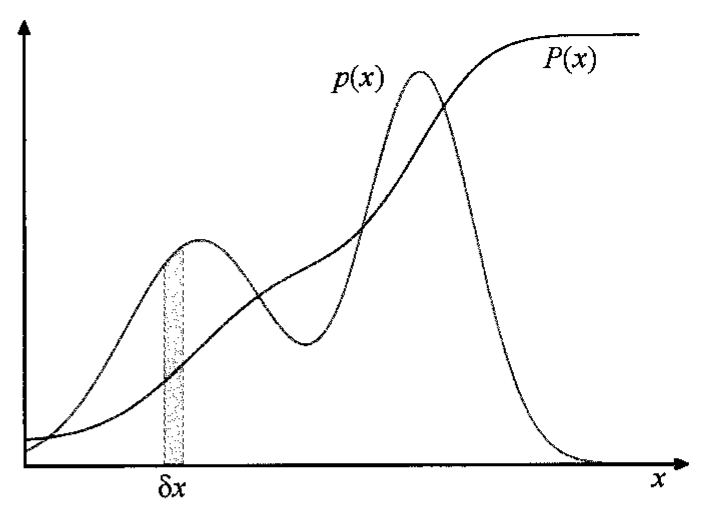
\includegraphics[width=0.58\textwidth]{ch02-fig2-6-density-cdf.png}
  \caption{离散变量下概率的概念可以推广到连续变量 $x$ 上的概率密度 $p(x)$，而当 $\delta x\to0$ 时，$x$ 落在区间 $(x,x+\delta x)$ 的概率由 $p(x)\delta x$ 给出。概率密度可以表示为累积分布函数 $P(x)$ 的导数。}
  \label{figure:ch02-密度与累积分布}
\end{figure}

因为概率是非负的，并且 $x$ 的值必须落在实轴上的某个位置，所以概率密度 $p(x)$ 必须同时满足以下两个条件：

\begin{align}
  p(x) \geqslant 0
  \label{align:ch02-密度非负}
\end{align}

\begin{align}
  \int_{-\infty}^{\infty} p(x)\,\mathrm{d}x = 1
  \label{align:ch02-密度归一化}
\end{align}

\begin{proposition}[概率密度的两个基本性质]\label{proposition:ch02-密度性质}
设 $p(x)$ 是\cref{definition:ch02-概率密度}意义下的概率密度，则它满足非负性\eqref{align:ch02-密度非负}与归一化条件\eqref{align:ch02-密度归一化}。
\end{proposition}

\begin{proof}
非负性：对任意 $x$ 与充分小的 $\delta x>0$，$p(x)\delta x$ 是事件 $\{x\in(x,x+\delta x)\}$ 的概率，概率非负而 $\delta x>0$，故 $p(x)\geqslant0$。

归一化：事件“$x$ 取实轴上的某个值”是必然事件，其概率为 $1$。把实轴分成互不重叠的小区间并求和，再令区间长度趋于零，由\eqref{align:ch02-区间概率}即得 $\int_{-\infty}^{\infty}p(x)\,\mathrm{d}x=1$。
\end{proof}

% SUPPLEMENT: parent=proposition:ch02-密度性质; kind=motivation; location=紧随其后的 remark（重构新增）
\begin{remark}（重构新增）
这两条性质正好对应概率公理中的两条：非负性保证不会算出负的概率，归一化保证全体可能取值的概率之和为 $1$。它们也是判断一个给定函数能否作为概率密度的唯一标准——\eqref{align:ch02-密度非负}与\eqref{align:ch02-密度归一化}同时成立即可。

归一化条件不可省：若只要求 $p\geqslant0$，则 $p(x)\equiv1$ 也会被当作密度，但它的积分发散，无法给出概率。原书把这类无法归一化的分布称为\textbf{反常}（improper）分布；在 Bayes 推断中，先验常常只在形式上给定、其归一化常数留到分母中处理，此时用的正是“未归一化的密度”。
\end{remark}

如\cref{figure:ch02-密度与累积分布}所示，$x$ 落在区间 $(-\infty,z)$ 的概率由累积分布函数（cumulative distribution function）给出，定义为

\begin{align}
  P(z) = \int_{-\infty}^{z} p(x)\,\mathrm{d}x
  \label{align:ch02-累积分布}
\end{align}

且满足 $P'(x)=p(x)$。

\begin{definition}[累积分布函数]\label{definition:ch02-累积分布函数}
称由\eqref{align:ch02-累积分布}定义的函数 $P(z)$ 为随机变量 $x$ 的\textbf{累积分布函数}（cumulative distribution function），它给出 $x$ 不超过 $z$ 的概率。
\end{definition}

% SUPPLEMENT: parent=definition:ch02-累积分布函数; kind=motivation; location=紧随其后的 remark（重构新增）
\begin{remark}（重构新增）
累积分布函数把“概率是多少”回答成“概率累积到哪里”：$P(z)$ 是密度在 $(-\infty,z]$ 上的积分，因此它单调不减、取值于 $[0,1]$，且 $z\to-\infty$ 时趋于 $0$、$z\to+\infty$ 时趋于 $1$。这三个性质正好是概率测度的三条公理在实轴上的体现。

与密度相比，$P$ 的好处是它总存在（任何随机变量都有分布函数），而密度不一定存在（例如离散变量或奇异分布）。\eqref{align:ch02-累积分布}用积分定义 $P$，因此隐含要求密度 $p$ 可积；对只有分布函数而没有密度的情形，本节的定义需要推广为 Stieltjes 积分。
\end{remark}

\begin{proposition}[累积分布函数的导数]\label{proposition:ch02-累积分布导数}
设概率密度 $p$ 在点 $x$ 处连续，$P$ 由\eqref{align:ch02-累积分布}定义，则 $P$ 在 $x$ 处可导且 $P'(x)=p(x)$。
\end{proposition}

\begin{proof}
由\eqref{align:ch02-累积分布}与\eqref{align:ch02-区间概率}，对 $h>0$，
\begin{align*}
  \frac{P(x+h)-P(x)}{h} = \frac{1}{h}\int_{x}^{x+h}p(t)\,\mathrm{d}t .
\end{align*}
当 $h\to0$ 时，右端是 $p$ 在 $[x,x+h]$ 上的平均值；由 $p$ 在 $x$ 处连续，该平均值趋于 $p(x)$。$h<0$ 的情形同理。故 $P'(x)=p(x)$。
\end{proof}

% SUPPLEMENT: parent=proposition:ch02-累积分布导数; kind=motivation; location=紧随其后的 remark（重构新增）
\begin{remark}（重构新增）
这条性质说明“密度”与“分布函数”是同一对象的两种描述：$P$ 是 $p$ 的积分，$p$ 是 $P$ 的导数。它的用途是把“求区间概率”转化为“求端点处的分布函数值之差”，即 $p(x\in(a,b))=P(b)-P(a)$，这在解析计算中往往更方便（例如\cref{section:ch03-周期变量}中处理周期变量时）。

条件“$p$ 在 $x$ 处连续”不可省：若 $p$ 在 $x$ 处有跳跃，$P$ 在该点不可导，只能断言 $P$ 在此处左、右导数分别等于 $p$ 的左、右极限。此外 $P$ 总是单调不减且 $\lim_{z\to-\infty}P(z)=0$、$\lim_{z\to+\infty}P(z)=1$，这两条由\eqref{align:ch02-密度非负}与\eqref{align:ch02-密度归一化}直接得到。
\end{remark}

假设有几个连续变量 $x_1,\cdots,x_D$，整体用向量 $\mathbf{x}$ 表示，我们可以定义联合概率密度 $p(\mathbf{x})=p(x_1,\cdots,x_D)$，使得 $\mathbf{x}$ 落在包含点 $\mathbf{x}$ 的无穷小体积 $\delta\mathbf{x}$ 中的概率由 $p(\mathbf{x})\delta\mathbf{x}$ 给出。该联合概率密度必须满足

\begin{align}
  p(\mathbf{x}) \geqslant 0
  \label{align:ch02-联合密度非负}
\end{align}

\begin{align}
  \int p(\mathbf{x})\,\mathrm{d}\mathbf{x} = 1
  \label{align:ch02-联合密度归一化}
\end{align}

其中积分是在整个 $\mathbf{x}$ 的空间上进行的。更一般地，我们还可以考虑同时包含离散变量和连续变量的联合概率分布。

\begin{definition}[联合概率密度]\label{definition:ch02-联合密度}
设 $\mathbf{x}=(x_1,\cdots,x_D)^{\mathsf{T}}$ 为 $D$ 维连续随机向量。若存在非负函数 $p(\mathbf{x})$，使得 $\mathbf{x}$ 落在包含点 $\mathbf{x}$ 的无穷小体积 $\delta\mathbf{x}$ 中的概率为 $p(\mathbf{x})\delta\mathbf{x}$，则称 $p(\mathbf{x})$ 为 $\mathbf{x}$ 的\textbf{联合概率密度}，并要求它满足\eqref{align:ch02-联合密度非负}与\eqref{align:ch02-联合密度归一化}。
\end{definition}

% SUPPLEMENT: parent=definition:ch02-联合密度; kind=motivation; location=紧随其后的 remark（重构新增）
\begin{remark}（重构新增）
联合密度是把\cref{definition:ch02-概率密度}逐维推广的结果：一维时 $\delta x$ 是长度，$D$ 维时 $\delta\mathbf{x}$ 是体积，因此 $p(\mathbf{x})$ 的量纲是“概率／体积”。\eqref{align:ch02-联合密度归一化}中的积分必须在整个 $\mathbf{x}$ 空间上进行，这是它与一维情形的唯一差别。

当 $D$ 很大时，联合密度所需的参数个数随 $D$ 迅速增长，直接建模不可行；这正是后文引入\cref{section:ch03-多元Gauss分布}中参数化形式（以及\cref{section:ch03-指数族分布}中指数族）的动机。
\end{remark}

概率的加和法则、乘积法则及 Bayes 定理，也适用于概率密度以及离散变量和连续变量的组合。如果 $x$ 和 $y$ 是两个实数变量，那么加和法则和乘积法则将有如下形式：

\begin{align}
  p(x) = \int p(x,y)\,\mathrm{d}y \quad \text{加和法则}
  \label{align:ch02-连续加和法则}
\end{align}

\begin{align}
  p(x,y) = p(y\mid x)\,p(x) \quad \text{乘积法则}
  \label{align:ch02-连续乘积法则}
\end{align}

类似地，Bayes 定理可以写成以下形式：

\begin{align}
  p(y\mid x) = \frac{p(x\mid y)\,p(y)}{p(x)}
  \label{align:ch02-连续Bayes}
\end{align}

其中分母由下式给出：

\begin{align}
  p(x) = \int p(x\mid y)\,p(y)\,\mathrm{d}y
  \label{align:ch02-Bayes分母连续}
\end{align}

\begin{theorem}[连续形式的加和法则、乘积法则与 Bayes 定理]\label{theorem:ch02-连续形式法则}
设 $x,y$ 为实值连续随机变量，其联合密度存在，则\eqref{align:ch02-连续加和法则}、\eqref{align:ch02-连续乘积法则}、\eqref{align:ch02-连续Bayes}与\eqref{align:ch02-Bayes分母连续}成立（其中\eqref{align:ch02-连续Bayes}要求 $p(x)>0$）。
\end{theorem}

\begin{proof}
把实轴划分为宽度为 $\Delta$ 的区间，将 $x$ 在第 $i$ 个区间、$y$ 在第 $j$ 个区间内的事件分别记为 $X=i$、$Y=j$。由\eqref{align:ch02-区间概率}，$\mathbb{P}(X=i)\approx p(x_i)\Delta$、$\mathbb{P}(X=i,Y=j)\approx p(x_i,y_j)\Delta^2$，其中 $x_i,y_j$ 为相应区间的代表点。这些离散事件满足\eqref{align:ch02-加和法则}与\eqref{align:ch02-乘积法则}，即
\begin{align*}
  \mathbb{P}(X=i) = \sum_{j}\mathbb{P}(X=i,Y=j),\qquad
  \mathbb{P}(X=i,Y=j) = \mathbb{P}(Y=j\mid X=i)\,\mathbb{P}(X=i) .
\end{align*}
把上述近似代入并约去公共因子 $\Delta$，得 $p(x_i)\approx\sum_j p(x_i,y_j)\Delta$ 与 $p(x_i,y_j)\approx p(y_j\mid x_i)p(x_i)$。令 $\Delta\to0$，求和过渡为积分，即得\eqref{align:ch02-连续加和法则}与\eqref{align:ch02-连续乘积法则}。再把\cref{theorem:ch02-Bayes定理}的推导逐字重复（把求和换成积分）即得\eqref{align:ch02-连续Bayes}与\eqref{align:ch02-Bayes分母连续}。
\end{proof}

% SUPPLEMENT: parent=theorem:ch02-连续形式法则; kind=motivation; location=紧随其后的 remark（重构新增）
\begin{remark}（重构新增）
这条定理的作用是宣布：前两节关于离散变量的全部法则，在连续情形下形式完全不变，只需把求和换成积分。因此后文讨论 Gauss 分布、密度变换与信息论时，可以不再区分离散与连续，只按需要选择求和或积分。

证明中的关键是“先离散化、再取极限”，而这个过渡的严格化需要测度论（Feller, 1966），超出了本书的范围；本书只要求上述法则在所用密度足够正则（例如分段连续）时成立。\eqref{align:ch02-连续Bayes}中的条件 $p(x)>0$ 不可省，理由与离散情形相同：分母出现在除法中。
\end{remark}

要对连续变量的加和法则和乘积法则做正式论证，需要借助名为测度论（measure theory）（Feller, 1966）的数学分支，这超出了本书的讨论范围。然而，通过将每个实变量划分为宽度为 $\Delta$ 的区间，并考虑这些区间上的离散概率分布，我们可以得知上述法则的正确性。通过取极限 $\Delta\to0$，然后求和转为积分，就可以得到我们想要的结果。

\subsection{分布的示例}\label{subsection:ch02-分布的示例}

很多形式的概率密度都得到了广泛应用，这些概率密度无论是它们本身还是作为更复杂概率模型的组件，都很重要。最简单的形式是 $p(x)$ 为常数，其独立于 $x$，但不能被归一化，因为\eqref{align:ch02-联合密度归一化}中的积分是发散的。不能被归一化的分布称为反常（improper）分布。然而，我们有这样的均匀分布，其在有限区间（比如 $(c,d)$）内是常数，而在其他地方为零。在这种情况下，\eqref{align:ch02-联合密度归一化}意味着

\begin{align}
  p(x) = \frac{1}{d-c}, \quad x\in(c,d)
  \label{align:ch02-均匀分布}
\end{align}

\begin{definition}[均匀分布]\label{definition:ch02-均匀分布}
设 $c<d$。称由\eqref{align:ch02-均匀分布}给出的概率密度为区间 $(c,d)$ 上的\textbf{均匀分布}（uniform distribution），即在 $(c,d)$ 内取常数、在区间外取零的密度。若某个密度在有限区间外为零、在区间内为常数，但其归一化常数尚未确定，则称相应的分布为\textbf{反常}（improper）分布。
\end{definition}

% SUPPLEMENT: parent=definition:ch02-均匀分布; kind=motivation; location=紧随其后的 remark（重构新增）
\begin{remark}（重构新增）
均匀分布是“在已知取值范围、而对取值本身一无所知”时最自然的密度：它把全部概率质量平均分配到区间上，是\cref{section:ch02-信息论}中最大熵原理在“支撑集有界”约束下给出的解。

常数 $1/(d-c)$ 完全由归一化确定，不可任意选取：若取其他常数，\eqref{align:ch02-密度归一化}便不成立。定义中对“反常分布”的说明提醒我们，常数密度在整条实轴上无法归一化，因此均匀分布必须限定在有限区间内；这也是后文使用无信息先验时需要格外小心的地方。
\end{remark}

概率密度的另一种简单形式是指数分布（exponential distribution），由下式给出：

\begin{align}
  p(x\mid\lambda) = \lambda\exp(-\lambda x), \quad x\geqslant 0
  \label{align:ch02-指数分布}
\end{align}

\begin{definition}[指数分布]\label{definition:ch02-指数分布}
设 $\lambda>0$。称由\eqref{align:ch02-指数分布}给出的概率密度为参数 $\lambda$ 的\textbf{指数分布}（exponential distribution），其支撑集为 $x\geqslant0$。
\end{definition}

指数分布有一种变体叫作 Laplace 分布（Laplace distribution），其允许将峰值移动到位置 $\mu$，由下式给出：

\begin{align}
  p(x\mid\mu,\gamma) = \frac{1}{2\gamma}\exp\left(-\frac{|x-\mu|}{\gamma}\right)
  \label{align:ch02-Laplace分布}
\end{align}

\begin{definition}[Laplace 分布]\label{definition:ch02-Laplace分布}
设 $\gamma>0$。称由\eqref{align:ch02-Laplace分布}给出的概率密度为参数 $\mu,\gamma$ 的 \textbf{Laplace} 分布（Laplace distribution），其中 $\mu$ 决定峰值的位置（对称中心），$\gamma$ 决定峰值的宽度。
\end{definition}

% SUPPLEMENT: parent=definition:ch02-指数分布; kind=motivation; location=紧随其后的 remark（重构新增）
% SUPPLEMENT: parent=definition:ch02-Laplace分布; kind=motivation; location=紧随其后的 remark（重构新增）
\begin{remark}（重构新增）
\cref{definition:ch02-均匀分布}、\cref{definition:ch02-指数分布}、\cref{definition:ch02-Laplace分布}这三个密度构成一个便于对照的序列：均匀分布在有界区间上“最平”，指数分布在半直线上单调衰减，Laplace 分布则以 $\mu$ 为中心、两侧对称地指数衰减。三者都由归一化常数唯一确定，而常数恰好等于“密度曲线下的面积”的倒数，因此\eqref{align:ch02-指数分布}中的 $\lambda$ 与\eqref{align:ch02-Laplace分布}中的 $2\gamma$ 都不是自由的。

条件 $\lambda>0$、$\gamma>0$ 不可省：若 $\lambda\leqslant0$，\eqref{align:ch02-指数分布}在 $x\to+\infty$ 时不衰减，积分为无穷；$\gamma$ 的情形同理。Laplace 分布中的绝对值 $|x-\mu|$ 保证两侧对称，若去掉绝对值，所得函数在 $\mu$ 处不连续且不再是关于 $\mu$ 对称的密度。指数分布可以看作 Laplace 分布在 $\mu=0$ 处只保留右半支的结果（此时归一化常数变为 $\lambda$ 而非 $1/(2\gamma)$）。
\end{remark}

\begin{figure}[htbp]
  \centering
  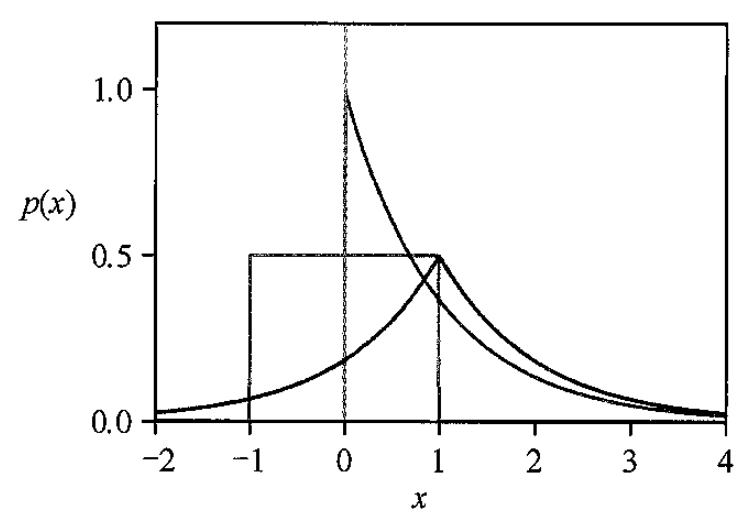
\includegraphics[width=0.55\textwidth]{ch02-fig2-7-uniform-exp-laplace.png}
  \caption{区间 $(-1,1)$ 内的均匀分布（红色），$\lambda=1$ 的指数分布（蓝色），以及 $\mu=1$ 和 $\gamma=1$ 的 Laplace 分布（绿色）的图示。}
  \label{figure:ch02-三种密度}
\end{figure}

均匀分布、指数分布和 Laplace 分布如\cref{figure:ch02-三种密度}所示。

另一个重要的分布是 Dirac $\delta$ 函数（Dirac delta function），由下式给出：

\begin{align}
  p(x\mid\mu) = \delta(x-\mu)
  \label{align:ch02-狄拉克}
\end{align}

\begin{definition}[Dirac $\delta$ 函数]\label{definition:ch02-狄拉克delta}
称满足“在除 $x=\mu$ 外的任意位置均为零、且积分为 $1$”的对象 $\delta(x-\mu)$ 为 \textbf{Dirac} $\delta$ 函数（Dirac delta function）。它可以视为位于 $x=\mu$ 处的无限窄且无限高的峰，并具有单位面积的性质，即
\begin{align*}
  \delta(x-\mu) = 0 \ (x\neq\mu), \qquad \int_{-\infty}^{\infty}\delta(x-\mu)\,\mathrm{d}x = 1 .
\end{align*}
\end{definition}

% SUPPLEMENT: parent=definition:ch02-狄拉克delta; kind=motivation; location=紧随其后的 remark（重构新增）
\begin{remark}（重构新增）
$\delta$ 函数把“概率质量集中在一点”这一极端情形也纳入了密度的语言：它的“密度”在 $\mu$ 处无穷大，但任何包含 $\mu$ 的区间上的积分都等于 $1$。正因为如此，离散分布与连续分布可以在同一个积分记号下统一处理，这是\cref{definition:ch02-经验分布}与后文混合模型的基础。

严格说来 $\delta$ 不是函数而是分布（广义函数），因此它不能像普通密度那样逐点求值，只能出现在积分号下。使用时必须保证积分区间包含 $\mu$，否则\eqref{align:ch02-狄拉克}的积分为零而非 $1$。
\end{remark}

最后，如果我们有一个 $x$ 的有限观测值集合 $\mathcal{D}=\{x_1,\cdots,x_N\}$，则可以使用 Dirac $\delta$ 函数来构造经验分布（empirical distribution），由下式给出：

\begin{align}
  p(x\mid\mathcal{D}) = \frac{1}{N}\sum_{n=1}^{N}\delta(x-x_n)
  \label{align:ch02-经验分布}
\end{align}

它由以每个数据点为中心的 Dirac $\delta$ 函数组成。根据要求，由\eqref{align:ch02-经验分布}定义的概率密度积分为 $1$（见\cref{exercise:ch02-06}）。

\begin{definition}[经验分布]\label{definition:ch02-经验分布}
设 $\mathcal{D}=\{x_1,\cdots,x_N\}$ 为一组观测值。称由\eqref{align:ch02-经验分布}给出的密度为这组数据的\textbf{经验分布}（empirical distribution），它把概率质量 $1/N$ 平均分配给每个观测点。
\end{definition}

% SUPPLEMENT: parent=definition:ch02-经验分布; kind=motivation; location=紧随其后的 remark（重构新增）
\begin{remark}（重构新增）
经验分布是“不对数据作任何分布假设”的建模方式：它只记录观测到了什么，而不假设数据来自某个参数族。因此它天然是\cref{subsection:ch02-分布的示例}末尾所说的反常密度的对立面——它一定是归一化的，但作为估计它并不光滑，且在观测点之外没有任何概率质量。

它的重要性在于把“对分布求期望”化为“对样本求平均”：由\cref{proposition:ch02-期望的样本近似}，$\mathbb{E}[f]\approx\frac{1}{N}\sum_n f(x_n)$。这也解释了为什么可以用样本均值估计期望，以及为什么样本量 $N$ 越大估计越可靠。
\end{remark}

\subsection{期望和协方差}\label{subsection:ch02-期望和协方差}

概率中最重要的操作之一是寻找函数的加权平均值。某函数 $f(x)$ 在概率分布 $p(x)$ 下的加权平均称为 $f(x)$ 的期望（expectation），用 $\mathbb{E}[f]$ 表示。对于离散分布，期望可以通过对所有可能值求和得到：

\begin{align}
  \mathbb{E}[f] = \sum_{x} p(x)\,f(x)
  \label{align:ch02-离散期望}
\end{align}

其中平均值由不同 $x$ 值的相对概率加权得到。对于连续变量，期望以相应的概率密度积分表示：

\begin{align}
  \mathbb{E}[f] = \int p(x)\,f(x)\,\mathrm{d}x
  \label{align:ch02-连续期望}
\end{align}

\begin{definition}[期望]\label{definition:ch02-期望}
设 $f$ 为随机变量 $x$ 的函数。称 $f(x)$ 在分布 $p(x)$ 下的加权平均为 $f(x)$ 的\textbf{期望}（expectation），记作 $\mathbb{E}[f]$；离散情形由\eqref{align:ch02-离散期望}定义，连续情形由\eqref{align:ch02-连续期望}定义（要求相应的和或积分绝对收敛）。
\end{definition}

% SUPPLEMENT: parent=definition:ch02-期望; kind=motivation; location=紧随其后的 remark（重构新增）
\begin{remark}（重构新增）
期望把“一个分布”压成一个数，因而是描述分布位置的最基本信息；它的定义方式（以概率为权重求和或积分）与中学的算术平均一致，只是权重由 $1/N$ 换成了 $p(x)$。\eqref{align:ch02-离散期望}与\eqref{align:ch02-连续期望}的差别仅在求和与积分，这正是\cref{theorem:ch02-连续形式法则}所保证的“形式不变”。

条件“绝对收敛”不可省：若 $\sum_x p(x)|f(x)|$ 发散，则期望可能依赖于求和次序而不唯一（例如 Cauchy 分布的均值），此时称期望不存在。本书讨论的分布都保证相应的和或积分收敛。
\end{remark}

不论在哪种情况下，如果我们从概率分布或概率密度中得到 $N$ 个有限数量的点，则期望可以近似为这些点的有限和（见\cref{exercise:ch02-07}）：

\begin{align}
  \mathbb{E}[f] \approx \frac{1}{N}\sum_{n=1}^{N} f(x_n)
  \label{align:ch02-样本近似}
\end{align}

\begin{proposition}[期望的样本近似]\label{proposition:ch02-期望的样本近似}
设 $x_1,\cdots,x_N$ 是来自分布 $p(x)$ 的样本，$\mathcal{D}=\{x_1,\cdots,x_N\}$，则关于经验分布\eqref{align:ch02-经验分布}的期望恰为样本平均，即
\begin{align*}
  \int f(x)\,p(x\mid\mathcal{D})\,\mathrm{d}x = \frac{1}{N}\sum_{n=1}^{N} f(x_n) ,
\end{align*}
从而当 $N\to\infty$ 时它依概率收敛到 $\mathbb{E}[f]$，这就是\eqref{align:ch02-样本近似}。
\end{proposition}

\begin{proof}
把\eqref{align:ch02-经验分布}代入并交换求和与积分（有限和，合法）：
\begin{align*}
  \int f(x)\,p(x\mid\mathcal{D})\,\mathrm{d}x
  = \frac{1}{N}\sum_{n=1}^{N}\int f(x)\,\delta(x-x_n)\,\mathrm{d}x
  = \frac{1}{N}\sum_{n=1}^{N} f(x_n) ,
\end{align*}
最后一步用到 $\delta$ 函数的定义。再由大数定律，样本平均依概率收敛到 $\mathbb{E}[f]$。
\end{proof}

% SUPPLEMENT: parent=proposition:ch02-期望的样本近似; kind=motivation; location=紧随其后的 remark（重构新增）
\begin{remark}（重构新增）
这条结果把“积分”变成了“求和”，是 Monte Carlo 方法的雏形：只要能从 $p(x)$ 中采样，就可以用样本平均近似任意函数的期望，而不必解析地计算积分。\eqref{align:ch02-样本近似}中的“$\approx$”在 $N\to\infty$ 时变为精确，误差的量级通常为 $O(N^{-1/2})$。

条件“样本来自 $p(x)$”不可省：若样本来自另一个分布 $q(x)$，则上式计算的是 $\mathbb{E}_q[f]$ 而非 $\mathbb{E}_p[f]$，两者的差别需要重要性采样来修正（参见\cref{section:ch14-基本采样}）。
\end{remark}

式\eqref{align:ch02-样本近似}中的近似在极限 $N\to\infty$ 下是精确的。

有时我们会考虑多个变量的函数期望，在这种情况下，我们可以使用下标来表示哪个变量被平均，例如

\begin{align}
  \mathbb{E}_{x}\big[f(x,y)\big]
  \label{align:ch02-偏期望}
\end{align}

这表示函数 $f(x,y)$ 相对于 $x$ 的分布的平均值。注意 $\mathbb{E}_{x}[f(x,y)]$ 是关于 $y$ 的函数。我们也可以考虑针对条件分布来说的条件期望（conditional expectation）：

\begin{align}
  \mathbb{E}_{x}\big[f\mid y\big] = \sum_{x} p(x\mid y)\,f(x)
  \label{align:ch02-条件期望}
\end{align}

$\mathbb{E}_{x}[f\mid y]$ 也是关于 $y$ 的函数。对于连续变量，条件期望的形式为

\begin{align}
  \mathbb{E}_{x}\big[f\mid y\big] = \int p(x\mid y)\,f(x)\,\mathrm{d}x
  \label{align:ch02-条件期望连续}
\end{align}

\begin{definition}[条件期望]\label{definition:ch02-条件期望}
设 $p(y)>0$。称 $f(x)$ 在给定 $y$ 的条件分布 $p(x\mid y)$ 下的平均值为 $f$ 关于 $x$ 的\textbf{条件期望}（conditional expectation），记作 $\mathbb{E}_x[f\mid y]$，离散情形由\eqref{align:ch02-条件期望}定义，连续情形由\eqref{align:ch02-条件期望连续}定义。类似地，$\mathbb{E}_x[f(x,y)]$ 表示 $f$ 关于 $x$ 的边缘分布的平均，见\eqref{align:ch02-偏期望}。
\end{definition}

% SUPPLEMENT: parent=definition:ch02-条件期望; kind=motivation; location=紧随其后的 remark（重构新增）
\begin{remark}（重构新增）
下标 $x$ 指出“对哪个变量求平均”，结果是剩余变量的函数；这一记号使“先对 $x$ 平均、再对 $y$ 平均”这类双重平均得以无歧义地书写，后文\cref{exercise:ch02-11}中的全期望公式与方差分解都要用到它。

条件期望与普通期望的差别在于所用的分布：\eqref{align:ch02-条件期望}用的是 $p(x\mid y)$ 而不是 $p(x)$，因此结果依赖 $y$。定义要求 $p(y)>0$，否则\eqref{align:ch02-条件期望}中的条件分布无定义——这与\cref{definition:ch02-条件概率}的要求一致。
\end{remark}

$f(x)$ 的方差（variance）定义为

\begin{align}
  \mathrm{var}[f] = \mathbb{E}\left[\big(f(x)-\mathbb{E}[f(x)]\big)^{2}\right]
  \label{align:ch02-方差}
\end{align}

\begin{definition}[方差]\label{definition:ch02-方差}
称由\eqref{align:ch02-方差}定义的量为 $f(x)$ 的\textbf{方差}（variance），它度量 $f(x)$ 围绕其均值 $\mathbb{E}[f(x)]$ 的分散程度。
\end{definition}

% SUPPLEMENT: parent=definition:ch02-方差; kind=motivation; location=紧随其后的 remark（重构新增）
\begin{remark}（重构新增）
方差是“二阶”的分散性度量：它先取偏差、再平方、最后平均，因此对大偏差的惩罚比对小偏差重。选择平方而非绝对值，是为了让方差可以展开成期望的代数式（见\cref{proposition:ch02-方差展开}），从而便于计算。

\eqref{align:ch02-方差}中的期望是对 $x$ 的分布取的，因此方差是一个数（不是函数）。方差恒非负；方差为零当且仅当 $f(x)$ 以概率 $1$ 取常数。
\end{remark}

式\eqref{align:ch02-方差}度量了 $f(x)$ 围绕其平均值 $\mathbb{E}[f(y)]$ 的变化程度。将平方项展开后，可以看到，方差也可以写成 $f(x)$ 和 $f(x)^2$ 的期望的形式（见\cref{exercise:ch02-08}）：

\begin{align}
  \mathrm{var}[f] = \mathbb{E}\left[f(x)^{2}\right] - \mathbb{E}\left[f(x)\right]^{2}
  \label{align:ch02-方差展开}
\end{align}

\begin{proposition}[方差的展开式]\label{proposition:ch02-方差展开}
设 $\mathbb{E}[f(x)^2]$ 存在，则\eqref{align:ch02-方差展开}成立。
\end{proposition}

\begin{proof}
记 $\mu=\mathbb{E}[f(x)]$，它是不依赖于 $x$ 的常数。把\eqref{align:ch02-方差}中的平方展开：
\begin{align*}
  \mathbb{E}\left[(f-\mu)^2\right] = \mathbb{E}\left[f^2 - 2\mu f + \mu^2\right] = \mathbb{E}[f^2] - 2\mu\,\mathbb{E}[f] + \mu^2 ,
\end{align*}
其中用到期望的线性性。代入 $\mathbb{E}[f]=\mu$ 得 $\mathbb{E}[f^2]-2\mu^2+\mu^2 = \mathbb{E}[f^2]-\mu^2$，即\eqref{align:ch02-方差展开}。
\end{proof}

% SUPPLEMENT: parent=proposition:ch02-方差展开; kind=motivation; location=紧随其后的 remark（重构新增）
\begin{remark}（重构新增）
此外，\eqref{align:ch02-方差}前正文中的 $\mathbb{E}[f(y)]$ 应为 $\mathbb{E}[f(x)]$（原书笔误，$y$ 在该句中并未出现），这不影响\eqref{align:ch02-方差}的表述。展开式的实际价值在于把“先算偏差再平方”换成“两个矩相减”，计算上少一次中心化；它也是后文证明方差可加性（\cref{exercise:ch02-10}）与协方差公式（\eqref{align:ch02-协方差矩阵}）的工具。

条件“$\mathbb{E}[f^2]$ 存在”不可省：若二阶矩不存在，\eqref{align:ch02-方差展开}右端两项可能同时为无穷，相减没有意义。另外该式的推导只用到期望的线性性，不要求 $x$ 离散或连续。
\end{remark}

变量 $x$ 自身的方差，其由下式给出：

\begin{align}
  \mathrm{var}[x] = \mathbb{E}\left[x^{2}\right] - \mathbb{E}[x]^{2}
  \label{align:ch02-变量方差}
\end{align}

对于两个随机变量 $x$ 和 $y$，协方差（covariance）度量了这两个变量一起变化的程度，定义为

\begin{align}
  \mathrm{cov}[x,y] &= \mathbb{E}_{x,y}\big[\{x-\mathbb{E}[x]\}\{y-\mathbb{E}[y]\}\big] \nonumber \\
  &= \mathbb{E}_{x,y}[xy] - \mathbb{E}[x]\,\mathbb{E}[y]
  \label{align:ch02-协方差}
\end{align}

\begin{definition}[协方差]\label{definition:ch02-协方差}
称由\eqref{align:ch02-协方差}第一行定义的量为随机变量 $x$ 与 $y$ 的\textbf{协方差}（covariance），记作 $\mathrm{cov}[x,y]$，它度量这两个变量一起变化的程度。当 $x=y$ 时 $\mathrm{cov}[x,x]=\mathrm{var}[x]$。
\end{definition}

% SUPPLEMENT: parent=definition:ch02-协方差; kind=motivation; location=紧随其后的 remark（重构新增）
\begin{remark}（重构新增）原文问题说明
\eqref{align:ch02-协方差}的第二行在原书中印作 $\mathbb{E}_{x,y}[xy]\,\mathbb{E}[x]\,\mathbb{E}[y]$，其中缺少减号。由第一行展开即可验证正确的等式为
\begin{align*}
  \mathbb{E}_{x,y}\big[\{x-\mathbb{E}[x]\}\{y-\mathbb{E}[y]\}\big]
  = \mathbb{E}_{x,y}[xy] - \mathbb{E}[x]\,\mathbb{E}[y] ,
\end{align*}
推导与\cref{proposition:ch02-方差展开}完全相同（把 $f$ 换成 $x$、把平方换成乘积）。若按原书字形理解，$\mathrm{cov}[x,y]$ 将等于三个非负数之积，与“协方差可以为负”这一基本事实矛盾，故此处按修正后的形式排版；下文\eqref{align:ch02-协方差矩阵}与\cref{proposition:ch02-独立协方差为零}均使用修正形式。
\end{remark}

\begin{remark}（重构新增）
协方差回答的是“两个变量是否同向变化”：当 $x$ 偏大时 $y$ 也偏大，乘积项为正，协方差为正；反向变化则为负。它与方差的关系 $\mathrm{cov}[x,x]=\mathrm{var}[x]$ 说明方差只是协方差在对角线上的特例，因此\eqref{align:ch02-协方差矩阵}可以把两者放进同一个矩阵。

$\mathrm{cov}[x,y]$ 的数值依赖 $x,y$ 的量纲，因此它的大小不能直接比较不同问题中的相关性强弱；这一点由相关系数（除以两个标准差）来弥补。定义要求二阶矩存在，理由与\cref{proposition:ch02-方差展开}相同。
\end{remark}

如果 $x$ 和 $y$ 是独立的，那么它们的协方差为零（见\cref{exercise:ch02-09}）。

\begin{proposition}[独立变量的协方差为零]\label{proposition:ch02-独立协方差为零}
若随机变量 $x$ 与 $y$ 独立，且二者的二阶矩存在，则 $\mathrm{cov}[x,y]=0$。
\end{proposition}

\begin{proof}
由独立性，$p(x,y)=p(x)p(y)$，故
\begin{align*}
  \mathbb{E}_{x,y}[xy] = \int\!\!\int xy\,p(x)p(y)\,\mathrm{d}x\,\mathrm{d}y
  = \left(\int x\,p(x)\,\mathrm{d}x\right)\left(\int y\,p(y)\,\mathrm{d}y\right) = \mathbb{E}[x]\,\mathbb{E}[y] .
\end{align*}
代入\eqref{align:ch02-协方差}的第二行即得 $\mathrm{cov}[x,y]=0$。
\end{proof}

% SUPPLEMENT: parent=proposition:ch02-独立协方差为零; kind=motivation; location=紧随其后的 remark（重构新增）
\begin{remark}（重构新增）
这条结论说明“独立”比“不相关”更强：独立可以推出协方差为零，反之不成立（\cref{exercise:ch02-39}给出了协方差为零但彼此依赖的反例）。因此在建模时，看到协方差为零不能直接断定变量无关。

证明中把二重积分拆成两个单重积分，关键仍是 $p(x,y)=p(x)p(y)$；若只知 $\mathrm{cov}[x,y]=0$，则 $\mathbb{E}[xy]=\mathbb{E}[x]\mathbb{E}[y]$ 成立，但推不出联合分布可分解。
\end{remark}

对于两个向量 $\mathbf{x}$ 和 $\mathbf{y}$，它们的协方差是由下式给出的矩阵：

\begin{align}
  \mathrm{cov}[\mathbf{x},\mathbf{y}] &= \mathbb{E}_{\mathbf{x},\mathbf{y}}\left[\big\{\mathbf{x}-\mathbb{E}[\mathbf{x}]\big\}\big\{\mathbf{y}^{\mathsf{T}}-\mathbb{E}[\mathbf{y}^{\mathsf{T}}]\big\}\right] \nonumber \\
  &= \mathbb{E}_{\mathbf{x},\mathbf{y}}\left[\mathbf{x}\mathbf{y}^{\mathsf{T}}\right] - \mathbb{E}[\mathbf{x}]\,\mathbb{E}[\mathbf{y}^{\mathsf{T}}]
  \label{align:ch02-协方差矩阵}
\end{align}

如果考虑向量 $\mathbf{x}$ 的分量彼此之间的协方差，则可以使用稍微简单一点的符号来表示：$\mathrm{cov}[\mathbf{x}]=\mathrm{cov}[\mathbf{x},\mathbf{x}]$。

\begin{definition}[协方差矩阵]\label{definition:ch02-协方差矩阵}
设 $\mathbf{x},\mathbf{y}$ 为随机向量。称由\eqref{align:ch02-协方差矩阵}定义的矩阵为 $\mathbf{x}$ 与 $\mathbf{y}$ 的\textbf{协方差矩阵}；当 $\mathbf{x}=\mathbf{y}$ 时简记 $\mathrm{cov}[\mathbf{x}]=\mathrm{cov}[\mathbf{x},\mathbf{x}]$，其第 $(i,j)$ 个元素是 $\mathrm{cov}[x_i,x_j]$。
\end{definition}

% SUPPLEMENT: parent=definition:ch02-协方差矩阵; kind=motivation; location=紧随其后的 remark（重构新增）
\begin{remark}（重构新增）
矩阵形式把 $\binom{D}{2}+D$ 个标量协方差打包成一个 $D\times D$ 矩阵，使得“线性变换下的协方差”可以用矩阵乘法表达（见\cref{section:ch03-多元Gauss分布}）。$\mathrm{cov}[\mathbf{x}]$ 必然是对称半正定矩阵，这一事实在\cref{section:ch03-多元Gauss分布}中决定多元 Gauss 分布的合法性。

\eqref{align:ch02-协方差矩阵}中的转置不可省：$\mathbf{x}\mathbf{y}^{\mathsf{T}}$ 是 $D\times D$ 矩阵，而 $\mathbf{x}^{\mathsf{T}}\mathbf{y}$ 是标量，二者含义完全不同。原书字形的第二行同样漏写了减号，修正方式与\eqref{align:ch02-协方差}相同，即第二行应为 $\mathbb{E}[\mathbf{x}\mathbf{y}^{\mathsf{T}}]-\mathbb{E}[\mathbf{x}]\,\mathbb{E}[\mathbf{y}^{\mathsf{T}}]$。
\end{remark}

\end{document}
